\documentclass[UTF8,a4paperdui, % draft
]{ctexart}
\usepackage[hidelinks]{hyperref}
\usepackage{bm}
\usepackage{graphicx}
\usepackage{pdfpages}
\usepackage{amsmath}
\usepackage{graphicx}
\usepackage{pdfpages}
\usepackage{amsmath}
\usepackage{cite}
\usepackage{caption,subcaption}
\usepackage{geometry}
\usepackage{pdfpages}
\usepackage[ruled,vlined,boxed,linesnumbered]{algorithm2e}
\usepackage{listings}
\usepackage{color}
\lstset {
  basicstyle=\small\ttfamily,
  captionpos=b,
  tabsize=2,
  columns=fixed,
  breaklines=true,
  frame=l,
  numbers=left,
  numberstyle=\small\ttfamily,
  morekeywords= {
    EQUAL, GREATER, LESS, NONE, SOME, abstraction, abstype, and, andalso, array, as, before, bool, case, char, datatype, do, else, end, eqtype, exception, exn, false, fn, fun, functor, handle, if, in, include, infix, infixr, int, let, list, local, nil, nonfix, not, o, of, op, open, option, orelse, overload, print, raise, real, rec, ref, sharing, sig, signature, string, struct, structure, substring, then, true, type, unit, val, vector, where, while, with, withtype, word
  },
  morestring=[b]",
  morecomment=[s]{(*}{*)},
  stringstyle=\color{black},
  identifierstyle=\color{eclipseBlue},
  keywordstyle=\color{red},
  commentstyle=\color{eclipseGreen}
}
\definecolor{eclipseBlue}{RGB}{42,0.0,255}
\definecolor{eclipseGreen}{RGB}{63,127,95}


\geometry{left=3.0cm,right=3.0cm,top=3cm,bottom=3cm}
%%%%%%%%%%%%%%%%%%%%%%%%%%%%
%%%%%%%%%%%%%%%%%%%%%%%%%%%%
\DeclareMathOperator{\net}{net}
\DeclareMathOperator{\sups}{SuperString}
%%%%%%%%%%%%%%%%%%%%%%%%%%%%
%%%%%%%%%%%%%%%%%%%%%%%%%%%%

\makeatletter
\algocf@newcmdside@kobe{LetIn@let}{%
\KwSty{let}%
\ifArgumentEmpty{#1}\relax{ #1}%
\algocf@group{#2}%
\par
}
\algocf@newcmdside@kobe{LetIn@in}{%
\KwSty{in}%
\ifArgumentEmpty{#1}\relax{ #1}%
\algocf@block{#2}{end}{#3}%
\par
}
\newcommand\LetIn[2]{%
\LetIn@let{#1}%
\LetIn@in{#2}%
}
\makeatother

\newcommand\op{\texttt{op}}
\newcommand\ttt{\texttt}
\newcommand\tbf{\textbf}
\newcommand\tit{\textit}
\newcommand\tttt[1]{\text{\ttt{#1}}}
\newcommand\givepar[2]{\ttt{)}$^{#1\ #2}$\ttt{(}}
\usepackage{amssymb}
\usepackage{extarrows}

\begin{document}
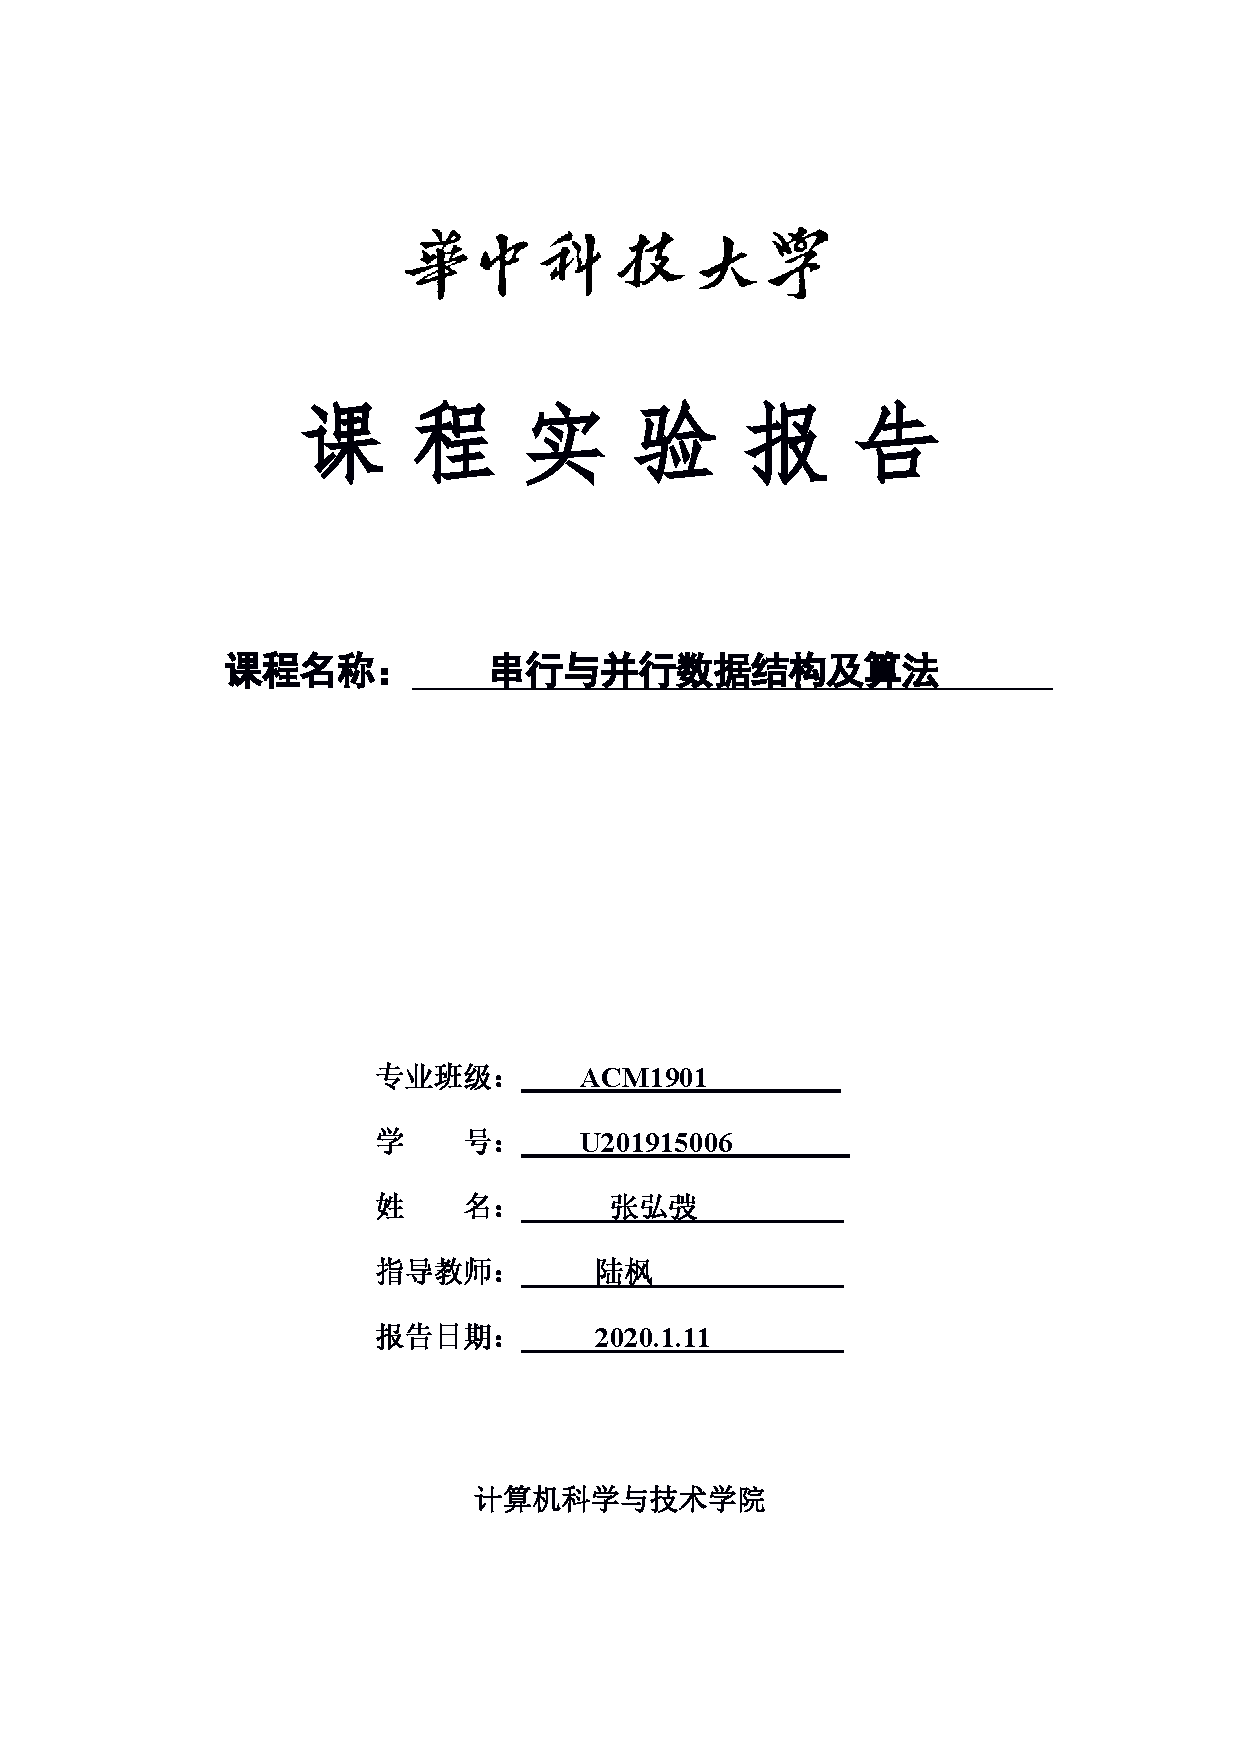
\includepdf[pages={1}]{cover.pdf}
\newpage
\newcommand*{\calF}{\mathcal{F}}
\newcommand*{\calH}{\mathcal{H}}
\newcommand*{\vx}{\bm x}
\newcommand*{\vy}{\bm y}
\newcommand*{\vh}{\bm h}
\newcommand{\Figure}[2]{
\begin{figure}[htbp]
\centering
\includegraphics[height=#1]{#2}
\end{figure}
}
%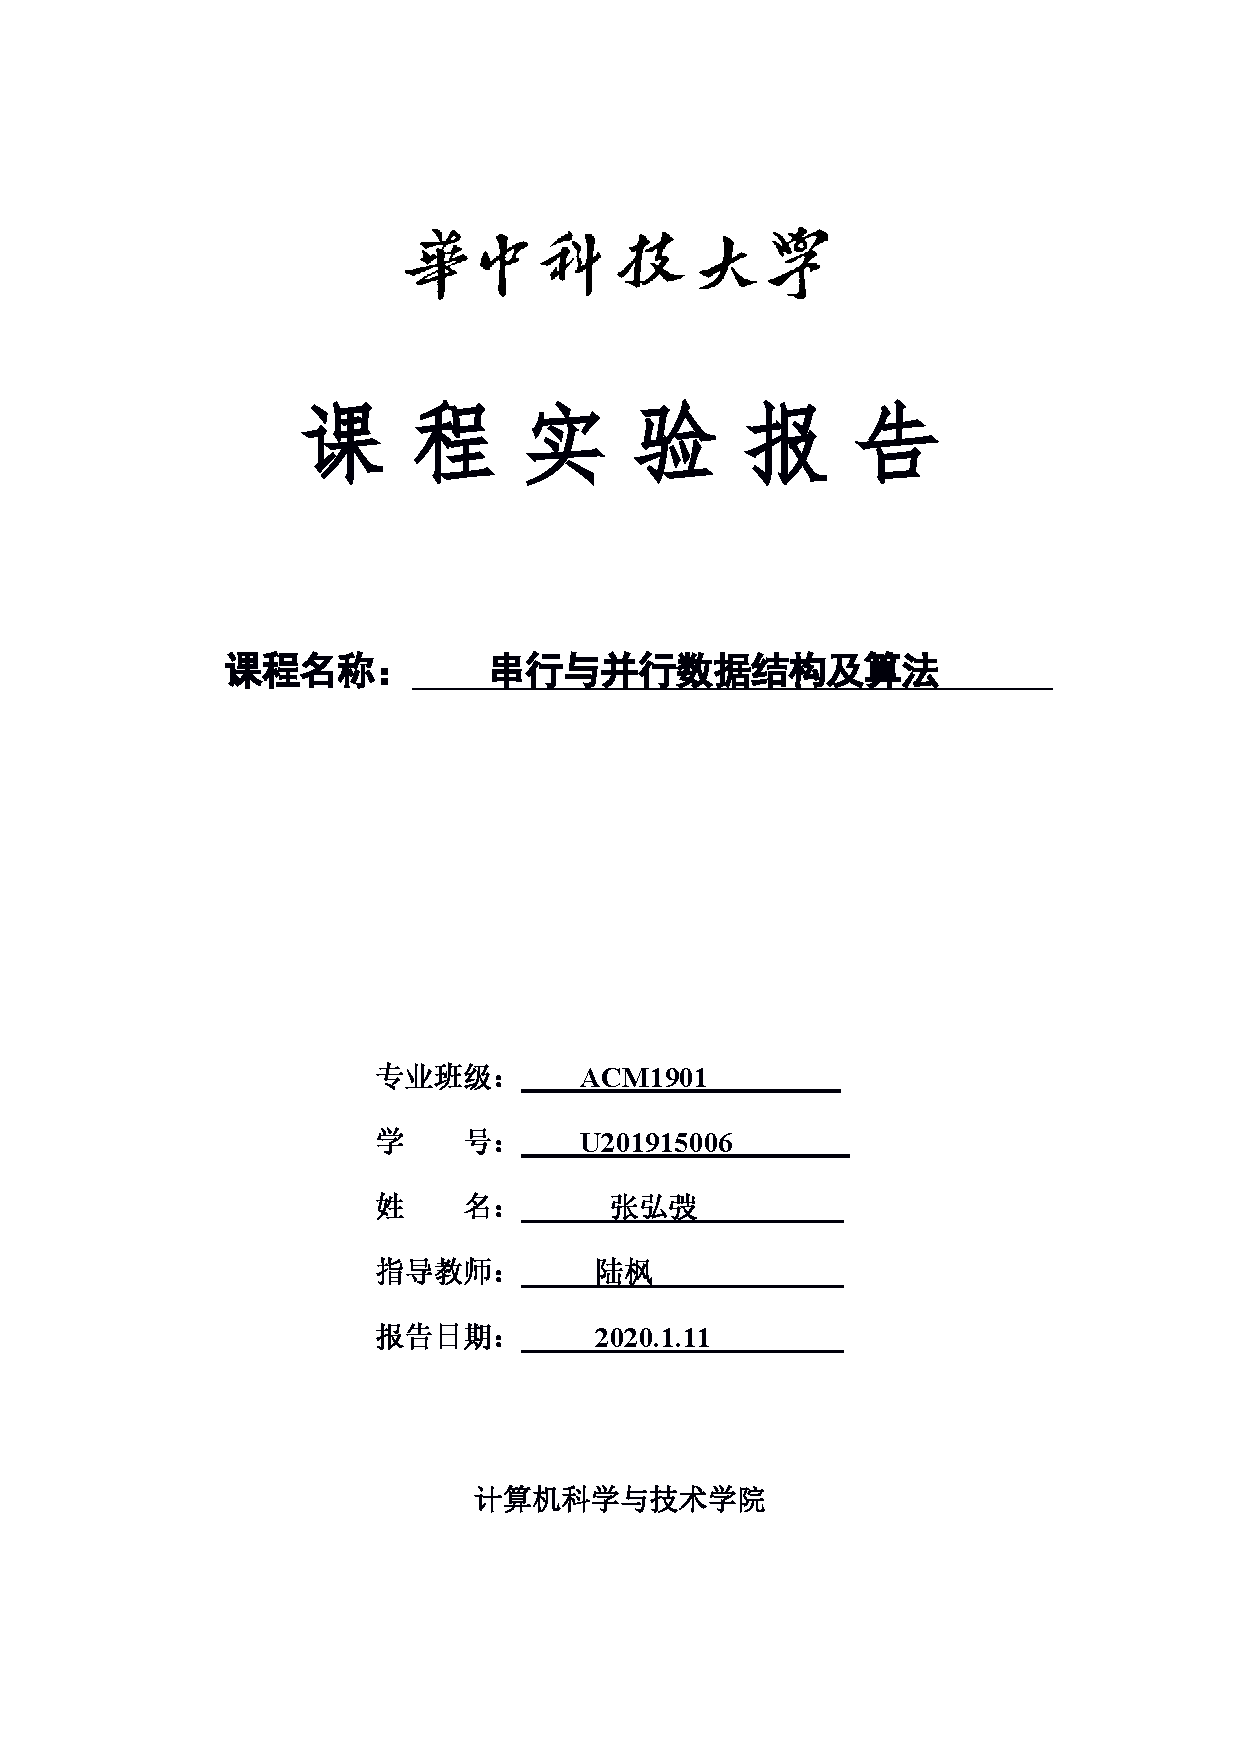
\includepdf{cover}
\tableofcontents
\newpage
\section{无重复排序}

\subsection{本关任务}
给出一个具有$N$个互不相同元素的数组,请对它进行升序排序。
\subsection{解法}
我们可以采用归并排序算法解决。

首先利用$\texttt{Mergesort}$将数据递归操作,首先将数据分为两半,再利用$\texttt{Merge}$进行归并。
\begin{algorithm}
\SetAlgoLined
MergeSort($\langle a_n\rangle$) =\par
\eIf{$|a_n|=1$}{$a_1$}{
\LetIn{
$L\longleftarrow $ MergeSort($\langle a_1,\ a_2,\ \ldots,\ a_{(n+1)/2}\rangle$)\;
$R\longleftarrow $ MergeSort($\langle a_{(n+1)/2},\ \ldots,\ a_{n}\rangle$)\;
}{
Merge($L, R$)}}
\caption{MergeSort}
\end{algorithm}

$\texttt{merge}$函数是对两个已经排序好的数字串进行排序,这样可以分为两种情况。第一种是两个数字串都不为空,那么直接比较两串头元素,较小的放在返回数字串的开头,再对剩下的数字串进行迭代操作。如果其中已经有一个数字串为空,那么直接返回剩下的所有数字串。因为每次返回的都是两个串中最小的元素,因此$\texttt{merge}$函数得到的数字串必定是从小到大有序排列的。


$\texttt{Mergesort}$首先利用$\texttt{sort}$函数将数字串分为两半,再利用$\texttt{merge}$进行两数字串的排序。$\texttt{sort}$(l, x)函数的两个参数分别是分出的左数字串的长度,和需要切分的数字串x,最后返回的就是排序好的字符串。在第6句中返回的x2已经是空值,而l2是已经排序好的子串。

\subsection{分析与证明}

证明:显然,当sort函数第一个参数值等于需要排序数字串的长度时,返回值的第二个值就为空,即返回的第一个值包含了所有需要排序的数。并且已经在前面证明了merge函数的正确性,因此只需证明l1,和l2是有序数列。

$sort(n, x)$返回值$(l, y)$,l是$x$的前$n$项的有序值,$y$是$x$的剩余项。当排序序列长度为1或2时显然成立。

假设,长度小于等于$k$的串经过$\texttt{sort}$函数的处理可以得到的是有序的串。

对于$k+1$长度的串来说,将会先分成两个长度为$(k+2)\ div\ 2$和$(k+1) div\ 2$的串排序,然后再通过$\texttt{merge}$操作归并。因此得到的$k+1$长度的串一定是有序的,证毕。

时间复杂度分析:在进行归并操作$\texttt{merge}$时需要的$W(n)=n$,$S(n)=logn$。假设对于一组数得拆分仅需要常数时间,因此得到$\texttt{Mergesort}$的递推公式$W(n)=2W(\frac{n}{2})+O(n)$,$S(n)=S(\frac{n}{2})+O(logn)$,计算得有
\[
W(n)=nlogn, S(n)=log^2n
\]

空间复杂度分析:在每一次进行$\texttt{merge}$排序时,都需要新的空间储存新生成的一组数。可以进行如下操作:首先开辟长度为$n$的空间储存所有通过$\texttt{merge}$操作排序的数(如下图所示),当排序好时就放到原来空间内。由于每一次并行操作时同一个数都不会同时出现在不同的$\texttt{merge}$操作中,因此不需要大于$n$的空间,因此空间复杂度为$O(n)$。

\begin{figure}[ht]
\centering
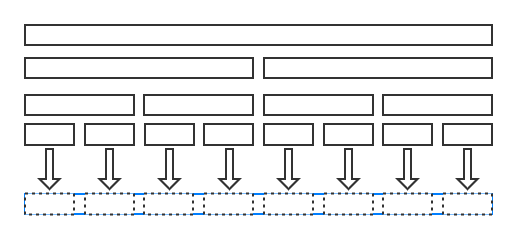
\includegraphics[scale=0.66]{空间.png}
\end{figure}

\subsection{样例输入与输出}
样例输入:

10

10 155 200 9 60 174 17 6 172 103

样例输出:

6 9 10 17 60 103 155 172 174 200 

样例分析:

首先将10个数分为两组数$\left \langle10,155,200,9,60\right \rangle ,\left \langle 174,17,6,172,103\right \rangle $,继续调用$\texttt{Mergesort}$,直到数组的长度为1或0。最后会被分解成如下图所示的情况。\\
\\
\\
\\
\\
\\
\\
\\
\begin{figure}[ht]
\centering
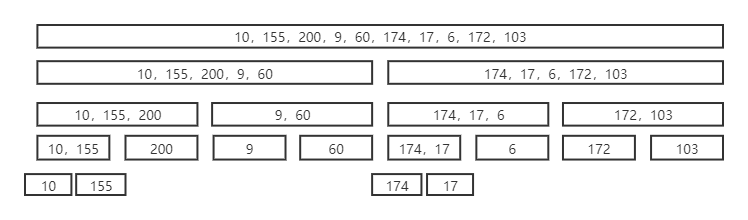
\includegraphics[scale=0.6]{1-example1.png}
\end{figure}

在分解到最后时,开始进行$\texttt{merge}$操作,即对每组有序数组进行再次排序。

%\begin{figure}[ht]
%\centering
%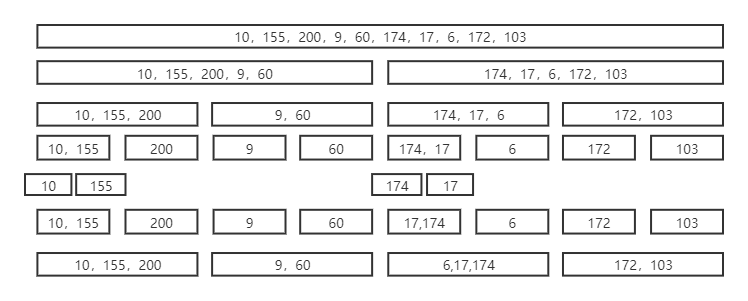
\includegraphics[scale=0.6]{1-example2.png}
%\end{figure}

\begin{figure}[ht]
\centering
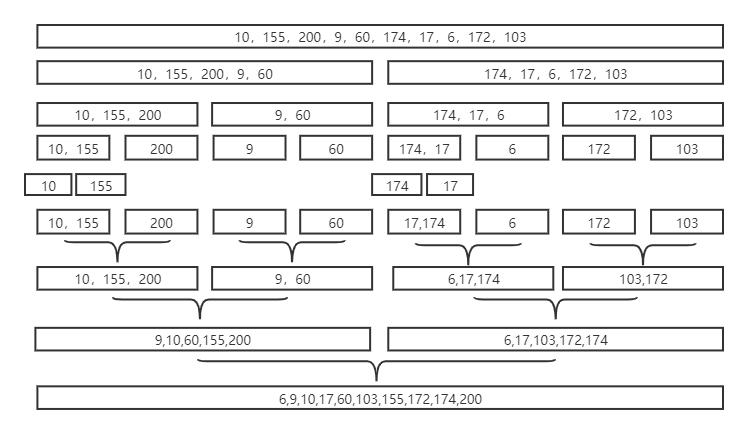
\includegraphics[scale=0.5]{1-example3.png}
\end{figure}

\section{最短路}
\subsection{本关任务}
给定一个带权无向图,一个源点,权值在边上。计算从源点到其他各点的最短路径。
\subsection{解法}
这里采用Dijkstra算法解决最短路问题。

利用邻接矩阵储存图。若无给定长度,则用$\infty$来表示无法两点之间无法到达。并创建一个命名为dis的sequence,用以储存源点到每个点的初始距离。创建一个集合B,B中最初只有源点。

(1)在dis数组中寻找一个长度最短的值dis[k],并且保证k点不在集合B中。

(2)对每个不属于B集合中的点进行长度收缩:如果dis[i]的值dis[k]+A[a][k]的大小,就将dis[i]的值更新为dis[k]+A[a][k]。将k也加入集合B中。

(3)重复上述步骤,直至集合B中包含所有点。得到的数组dis的值就是源点到所有对应点的最短路径值。

在最后输出最短路之前,再将所有长度为99999(表示$\inf$)的数据转化成~1说明没有此路径。

伪代码如下:
\begin{algorithm}
\SetAlgoLined
Dijstra($\langle G\rangle$) =\par
\LetIn{
$dijstra\ X\ S$ =\par
\eIf{$|s|=0$}
{$X$}
{\LetIn{
$v=deleteMin\ S$\par
$X'=X\cup \{v\}$\par
$G'=iterate\ relax\ G\ (N_G^+(v))$}{$dijstra\ X'\ G'$}}
}{
$dijstra\ \{\}\ s_0$ \ \ \ \ \ \ \ \ \ \ \ (*$s_0$为源点*)}
\caption{Dijstra}
\end{algorithm}
\subsection{分析与证明}
假设利用最小堆来存储源点到各点的距离。

时间复杂度分析:Dijkstra算法在一共进行$|V|$次步骤(1),在寻找长度最短值并维护堆时,需要的复杂度是$W=O(log|V|)$,$S=O(log|V|)$。选定最短长度后,开始对其他边进行收缩操作,因为要进行$|V|$次比较和更新长度,串行复杂度是$O(|V|)$,并行复杂度是$O(1)$。因此总的串行复杂度为$O(n^2)$。每一次的迭代都不能并行运算,因此并行复杂度$S=n^2$。由于两点之间本来没有通路,可能经过收缩可以通过,因此在分析时也将其算作一个临界点,即有$|E|=|V|^2$。如果没有这个条件,Dijkstra的复杂度为$W=O(|E|log|V|),S=O(|E|log|V|)$。

证明:最小堆的删除操作需要$O(logn)$,\texttt{union}操作需要$O(logn)$的复杂度,收缩长度使用迭代操作需要$O(n)$,得到递推式$T(n)=T(n-1)+2logn+n$,解得$T(n)=2logn!+\frac{n(n+1)}{2}$
\[
\lim\limits_{n\rightarrow \infty}{\frac{logn!}{logn^n}}=\lim\limits_{n\rightarrow \infty}{\frac{log(\sqrt{2\pi n}(\frac{n^n}{e^n}))}{nlogn}}
\]
\[=\lim\limits_{n\rightarrow \infty}{\frac{\frac{1}{2}log(2\pi)+\frac{1}{2}logn+nlogn-nloge}{nlogn}}=\lim\limits_{n\rightarrow \infty}{\frac{\frac{1}{2}log(2\pi)}{nlogn}+\frac{1}{2n}+1-\frac{1}{lnn}}=1
\]
因此$0\leq T(n)\leq 2nlogn+\frac{n^2}{2}+\frac{n}{2}$。
对于并行时间复杂度,有$T(n)=T(n-1)+1+logn+n$,$S(n)\in O(N^2)$
因此
\[
W(n)=n^2,S(n)=n^2
\]

空间复杂度分析:该算法利用邻接矩阵存储,空间复杂度为$O(|V|^2)$,利用sequence来实现最小堆,存储源点到各点长度时,空间复杂度为$O(|V|)$。因此总的空间复杂度为$O(|V|^2)$。

\subsection{样例输入与输出}
样例输入:

7 11 5

2 4 2

1 4 3

7 2 2

3 4 3

5 7 5

7 3 3

6 1 1

6 3 4

2 4 3

5 6 3

7 2 1

样例输出:

4 6 7 7 0 3 5 

样例分析:

首先得到邻接矩阵:
\[
\left[
    \begin{array}{ccccccc}
        0 & \infty & \infty & 3 & \infty & 1 & \infty \\
        \infty & 0 & \infty & 2 & \infty & \infty & 1 \\
        \infty & \infty & 0 & 3 & \infty & 4 & 3 \\
        3 & 2 & 3 & 0 & \infty & \infty & \infty \\
        \infty & \infty & \infty & \infty & 0 & 3 & 5 \\
        1 & \infty & 4 & \infty & 3 & 0 & \infty \\
        \infty & 2 & 3 & \infty & 5 & \infty & 0
    \end{array}
\right]
\]

dis数组数值为
\[
\left[
	\begin{array}{ccccccc}
		\infty & \infty & \infty & \infty & 0 & 3 & 5
	\end{array}
\right]
\]

首先将源点5加入$X$集合中。

选取距离源点最短的点6,对除$X$集合外的所有点$w$进行收缩,$dis[w]=min\{G[w][6]+dis[6],dis[w]\}$,以此更新dis数组。

得到收缩后的结果为
\[
\left[
	\begin{array}{ccccccc}
		4 & \infty & 7 & \infty & 0 & 3 & 5
	\end{array}
\right]
\]

下面步骤同理,最后得到dis函数数值为
\[
\left[
	\begin{array}{ccccccc}
		4 & 6 & 7 & 7 & 0 & 3 & 5
	\end{array}
\right]
\]
\section{最大括号距离}
\subsection{本关任务}
我们定义一个串s是闭合的,当且仅当它由'('和')'构成,而且满足以下条件之一:

空串:这个串为空

连接:这个串由两个闭合的串连接构成

匹配:这个串是一个闭合的串外面包裹一个括号构成的

现在给你一个串,你需要找出所有这个串中匹配的子串(一个闭合的串,并且外侧由括号包裹)中最长的那个,输出它的长度。
\subsection{解法}
使用一个模拟栈的函数来储存左括号序号。

当栈为空时,判断下一个要入栈的括号的类型:如果是右括号,则必定不会有与之匹配的括号,直接跳过右括号;如果是左括号,就将左括号的序号压栈。并在每次栈为空时更新当前最大的匹配括号长度。

当栈不为空时,若扫描到的是左括号,继续将左括号的序号压栈。如果是右括号,即右括号和栈顶的左括号匹配,将栈顶序号弹出,两括号的距离即是两序号之差,与当前括号最大距离进行比较,并更新最大括号距离。


\subsection{分析与证明}
关键函数stack的代码如下:

时间复杂度分析:该算法对一串括号进行线性扫描操作,因此并行复杂度与串行复杂度相等。在扫描每一个括号时,都要对括号类型进行判断,进行压栈、更新最大距离等操作,都需要常数时间,因此时间复杂度只与括号串的长度有关。时间复杂度为$W=O(n),S=(n)$。

证明:

此算法无法并行处理,串行时间复杂度和并行时间复杂度相同。有递推式$T(n)=T(n-1)+1$,因此有
\[
	W(n)=O(n),S(n)=O(n)
\]

空间复杂度分析:$\texttt{stack}$函数的第一个参数和第二个参数都至多需要储存长度为$n$的序列,因此空间复杂度为$O(n)$。此空间复杂度易证。

\subsection{样例输入与输出}
样例输入:

12 

1 0 1 0 1 1 0 0 1 0 1 1

样例输出:

6

样例分析:

第一个扫描到的括号是右括号,直接舍去。下一个括号是左括号,在栈中储存位置$[1]$,扫描到的下一个括号是右括号,计算当前匹配的距离为$2-1+1=2$,更新最大匹配距离为2。在扫描到第八个位置时候,栈中元素为$[8,7]$。下一个是右括号,栈弹出一个元素,此处括号距离为2,不更新最长括号距离。下一个是左括号,将其位置入栈,$[10,7]$,依次类推,在扫描到最后一个括号时,计算其距离为$12-7+1=6$。因此此括号串最大距离为6。
\section{天际线}
\subsection{本关任务}
城市的天际线是从远处观看该城市中所有建筑物形成的轮廓的外部轮廓。现在,假设您获得了城市风光照片上显示的所有建筑物的位置和高度,请编写一个程序以输出由这些建筑物形成的天际线。

每个建筑物的几何信息用三元组 $[\ L_i,\ H_i,\ R_i]$ 表示,其中 $L_i$ 和 $R_i$ 分别是第 $i$ 座建筑物左右边缘的 $x$ 坐标,$H_i$ 是其高度。可以保证 $0 \leq L_i$, $R_i \leq  {\rm INT\_MAX}$, $0 < Hi \leq  {\rm INT\_MAX}$ 和 $Ri - Li > 0$。您可以假设所有建筑物都是在绝对平坦且高度为 0 的表面上的完美矩形。

输出是以$[\ [\ x_1,\ y_1],\ [\ x_2,\ y_2\ ],\ [x_3,\ y_3],\ ...\ ]$ 格式的“关键点”的列表,它们唯一地定义了天际线。关键点是水平线段的左端点。请注意,最右侧建筑物的最后一个关键点仅用于标记天际线的终点,并始终为零高度。此外,任何两个相邻建筑物之间的地面都应被视为天际线轮廓的一部分。
\subsection{解法}
可以使用分治方法解决问题。

三元组$[\ L_i,\ H_i,\ R_i\ ]$可以看成一个基础轮廓,即$[(L_i, H_i), (R_i, 0)]$。读入所有数据,即有$n$组基础轮廓。

\begin{algorithm}
\SetAlgoLined
Skyline($G$) =\par
\eIf{$|G|=0\ or\ |G|=1$}{$G$}{
\LetIn{
$merge\ G_1\ G_2\ X$ =\par
\eIf{$|G_1|=0\ and\ |G_2|=0$}
{$X$}
{\LetIn{
$(x',\ h')={\arg\min}_{(x,\_)\in \tau}G_1\cup G_2$\par
$X'=\ Add\ X\  \{(x',\ h')\}$\par
$G_1'=G1\ \backslash \ \{(x',\ h')\}$\par
$G_2'=G2\ \backslash \ \{(x',\ h')\}$\par
}{$merge\ G_1'\ G_2'\ X'$}}
$G_1\longleftarrow G[0,1,...,|G|/2]$\par
$G_2\longleftarrow G[|G|/2+1,...,|G|-1]$
}{
$merge\ G_1\ G_2$}}
\caption{Skyline}
\end{algorithm}


(1)当轮廓数为1或0时,直接返回该轮廓。

(2)当轮廓数大于等于2时,将其分成两组轮廓,分别进行组合。


Merge操作是对两个轮廓,$S1$和$S2$进行合并。

设h1,h2分别为两个轮廓当前的高度,$x1$和$x2$分别为未处理的两个串的横坐标,用变量$last$表示最后一个加入新轮廓的高度。

如果$x1\ >\ x2$,将$h2$更新为$x2$对应的高度。将$(x2, max(h1, h2))$加入新轮廓,如果last值与x2对应的高度不相等。

同理,若$x1\ <\ x2$,将$h1$更新为$x1$对应的高度。将$(x1, max(h1, h2))$加入新轮廓,如果last值与$x1$对应的高度不相等。

当$x1\ =\ x2$,也有相同的操作。


\subsection{分析与证明}

在拆分轮廓时仅需要常量时间。当两个长度为n的轮廓进行合并时,需要线性扫描两轮廓,在处理时也需要常数时间,时间复杂度为$O(2n)$,得到递推式$W(n)=2W(\frac{n}{2})+O(n)$。$W(n)=2W(\frac{n}{2})+O(n)=4W(\frac{n}{4})+O(n)+2O(\frac{n}{2})=\sum_{i=0}^n{2^i\cdot \frac{n}{2^{i}}}=nlogn$。每一个合并操作都可以并行进行处理,即通过并行处理的方法将$G_1$、$G_2$的坐标以坐标大小进行排序,再去除其中相邻的高度的坐标。去除的这一步骤只需要常数时间,因此时间复杂度为$O(logn)$,递推式为$S(n)=S(\frac{n}{2})+logn$,因此$S(n)=log^2n$。

对于所需空间,首先储存读入数据需要$O(2n)$的空间,在每次Merge操作中都需要创建新的空间存储处理的数据,而对于每一层的拆分并不需要每次都开辟新的空间,在最初直接开辟$O(2n)$的空间进行所有Merge操作就足够。因此空间复杂度为$O(n)$。


\subsection{样例输入与输出}
样例输入:

4

1 3 4

3 2 11

6 6 8

7 4 10
\\

样例输出:

1 3 

4 2 

6 6 

8 4 

10 2 

11 0 
\\

样例分析:

最初储存的天际线组是$[[(1,3),(4,0)],[(3,2),(11,0)],[(6,6),(8,0)],[(7,4),(10,0)]]$。经过拆分,首先merge前两组天际线:$[(1,3),(4,0)]$和$[(3,2),(11,0)]$。首先,$h_1=0,h_2=0$。选择横坐标最小的(1,3),更新$h_1$为3,因此得到的第一个轮廓点的高度为$\max\{h_1,h_2\}=\max\{3,0\}=3$。再选择当前横坐标最小的点(3,2),高度$H=\max\{h_1,h_2\}=\max\{3,2\}=3$,应该添加(3,2)。但是由于该点高度与前一个点相同,即是天际线中的中间点,所以不添加,直接开始处理下一个点。同理,得到前两个天际线组的组合结果是$[(1,3),(4,2),(11,0)]$。后两个天际线组的组合结果是$[(6,6),(8,4),(10,0)]$,最后的$\texttt{merge}$结果即为样例输出结果。
\section{括号匹配}
\subsection{本关任务}
给定一个括号序列,判断它是否是匹配的。注意( ) ( ) 在本题也当做匹配处理。
\subsection{解法}
定义左括号为1,右括号为-1。从左至右进行加法,初始值为0。如果在计算过程中中间过程小于零,则括号序列不匹配,如果最后结果不为零,括号序列也不匹配。
\begin{algorithm}
  \SetAlgoLined
  MatchPar($L$) =\par
    \LetIn{
      $(a,b)=scan\ +\ 0\ L$\par
      $val\ flag\ =\ $\par
      \eIf{$b\ !=\ 0$}{$0$}{
        \eIf{$(filter\ (fn\ x\ =>\ x\ <\ 0)\ a)\ !=\ [\ ]$}
      {0}{1}}     
    }{flag}
  \caption{MatchPar}
\end{algorithm}
\subsection{分析与证明}
时间复杂度:此算法采用线性扫描的方式来处理括号串,并返回每一个过程。根据书本,$\texttt{scan}$操作需要花费$Work$为$O(n)$,$S$为$O(logn)$。而$\texttt{filter}$操作也是需要线性长度的时间,因此此算法的时间复杂度为
\[
  W=O(n),\ S=O(logn)
\]


空间复杂度:处理长度为$n$的括号串,需要储存的空间是$n+1$的空间去储存扫描到每一个元素加法的结果。因此需要$O(n)$的空间。
\subsection{样例输入与输出}
样例输入:

18

0 0 0 0 1 1 0 0 1 0 1 1 0 0 1 1 1 1

样例输出:

1

样例分析:

用$\texttt{scan}$操作来扫描整个括号串,得到的结果为$(\langle 0,1,2,3,4,3,2,3,4,3,4,3,2,3,4,3,2,1\rangle ,0)$。由于元组的第二个元素为0,并且第一个元素中的所有数都不为负数,因此该括号串匹配。


\section{高精度整数}
\subsection{本关任务}
给定两个任意精度的整数a和b,满足a$\geq$b,求出a+b, a−b, a×b的值。
\subsection{解法}
\subsubsection{加法的计算}
将两个数列进行翻转,即将两个数的最后一位对齐,做相应的加法。

如果两个数相加大于9,就将$c$置为1,在下一位上加上1。
\begin{figure}[ht]
\centering
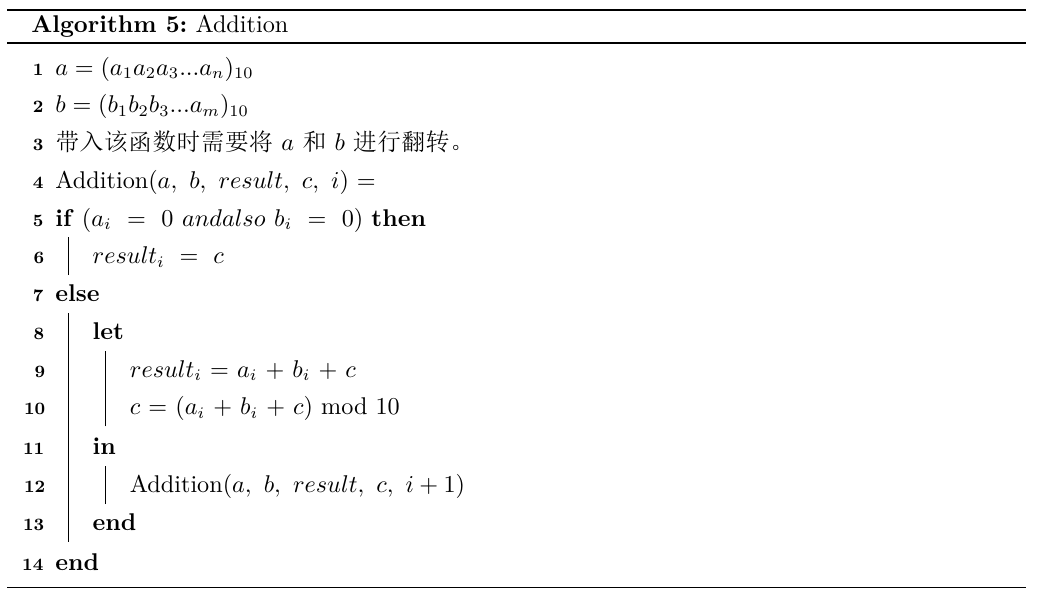
\includegraphics[scale=0.57]{Addition.png}
\end{figure}

\subsubsection{减法的计算}
减法的计算与加法同理,也是将最后一位对齐,从低位开始相减。并用$c$来表示在下一位是否要退位,如果$a-b<0$。
算法如下。
\begin{figure}[ht]
\centering
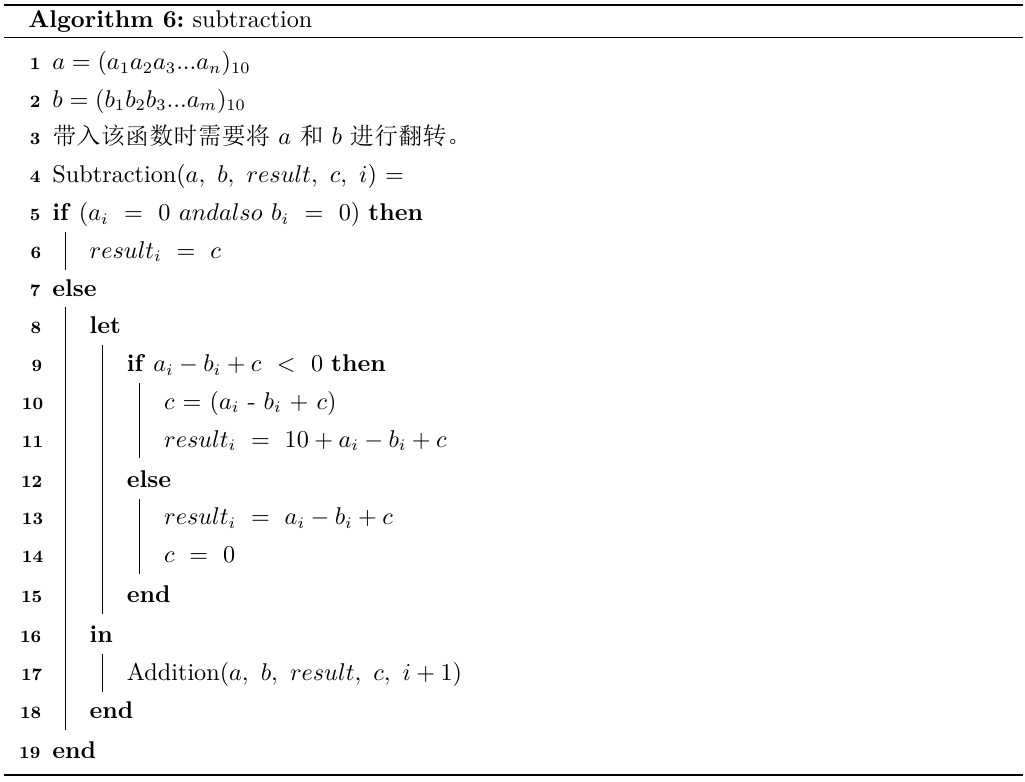
\includegraphics[scale=0.56]{Substraction.png}
\end{figure}



\subsubsection{乘法的计算}
先将多位数相乘转换为多个一位数与多位数相乘的乘法。

与上述加法和减法的操作类似,从最末位开始相乘,并用$c$来记录下一位的进位数。

对于第$k$位数完成乘法运算后还要在末尾加上$k-1$个零。

再将所有得到的结果相加。

\begin{lstlisting}
fun onemultiply(a, [], c) = [c]
  | onemultiply(a, b::bs, c) = 
        if (a * b + c> 9) then ((a*b+c)mod 10)::onemultiply(a, bs, (a*b+c) div 10)
                          else (a*b+c)::onemultiply(a, bs, 0);
fun multiply([], bs) = [0]
  | multiply(a::ass, bs) = 
        Add(onemultiply(a, bs, 0), 0::multiply(ass, bs), 0);
\end{lstlisting}


\subsection{分析与证明}
对于加法来说, $n$和$m$相加,需要对应扫描两数的每一位数,需要的串行时间与两个数的最长位数成线性关系。$W=O(max(|logn|,\ |logm|)+1)\in O(logn)$对于最优并行算法来说,可以用$\texttt{map}$操作对对应位数的两个数字相加,并记录每一位需要进位的个数。再将进位数相应相加。重复操作,直到所有每一位的进位数都为0。因此并行算法的复杂度$S=O(loglogn)$。

减法与加法同理,有同样的串行复杂度W。

乘法的算法是加法的叠加,将一个数的每一位对另一个数相乘,再将得到的结果相应进位相加。对于每一位和另一个数相乘的操作,需要的$W=O(logn),S=O(log(logn))$。在将最后得到的结果相加时,根据加法复杂度的分析,得到$W=O(nlogn),S=O(logn\cdot log(logn))$。
因此加法的总的复杂度为
\[
W=O(nlogn),S=O(logn\cdot log(logn))
\]
\subsection{样例输入与输出}
样例输入:

10

2 3 3 3 3 3 3 3 3 3 
 
10 

2 3 3 3 3 3 3 3 3 3

样例输出:

4 6 6 6 6 6 6 6 6 6 

0 

5 4 4 4 4 4 4 4 4 2 8 8 8 8 8 8 8 8 9 

样例分析:

将两数字串$[3,3,3,3,3,3,3,3,3,2]$,$[3,3,3,3,3,3,3,3,3,2]$。

按位进行加法,有$[6,6,6,6,6,6,6,6,6,4]$。

按位减法,$[0,0,0,0,0,0,0,0,0,0]$,由于所有位数为0,只输出一位0。

乘法法运算时,得到第一位数与另一数乘法的结果$[9,9,9,9,9,9,9,9,9,6]$。第二位数结果为$0::[9,9,9,9,9,9,9,9,9,0]$。第三位为$0::0::[9,9,9,9,9,9,9,9,9,6]$。将每一位的乘法的结果调用加法运算即可。
\section{割点与割边}
\subsection{本关测试}
给定一个无向无权连通图,请求出这个图的所有割点和割边的数目。
\subsection{解法}
利用Tarjan算法进行实现。
定义两个数组,dfn[ ], low[ ]。

dfn[ ]表示对应节点在深度优先搜索时遍历的时间戳,每访问到一个新节点时间戳增加1。

每个节点被第一次访问时,low值与dfn值相同。当继续访问相邻节点,满足邻节点的low值小于节点low值,并且邻节点并不是父亲节点,则更新节点low值,并在回退中更新所有的low值。因此low表示了不通过父节点所能访问到的最早祖先节点。

深度优先搜索结束后,对图中每一个顶点U,以及它的所有的孩子顶点low值进行比较,如果至少存在一个孩子顶点V满足$low[v]\geq dfn[u]$,说明顶点V必须通过顶点U访问U的祖先节点,说明U时一个割点。

当满足low[v] $>$ dfn[u],说明V-U是桥。

\subsection{分析与证明}
时间复杂度分析:已经知道,每次low和dfn数组的更新只需要常数时间。对于深度优先搜索,可以通过栈的实现方式去理解。如果碰到了一个未被访问过的节点(即dfn对应值为0),那么就入栈,并将它所有顶点依次入栈。对于已被访问过的元素,则更新与之相连的所有点的low值。由于有$|V|$个节点,$|E|$条边,每个节点会入栈一次,每次对于已访问过的节点向前更新low值得次数小于等于边的个数。如果用邻接表的方式储存图,搜索相邻点需要的时间也为常数时间,因此时间复杂度为$O(|V|+|E|)$。由于无法进行并行操作,并行时间复杂度也为$O(|V|+|E|)$。

算法需要的空间复杂度主要用于储存low、dfn数组,需要$O(|V|)$的空间。与时间复杂度对应,使用邻接表来储存整张图,需要$O(|V|+|E|)$的空间。因此总的空间复杂度为$O(|V|+|E|)$。
\subsection{样例结果与输出}
样例输入:

10 12 

1 2 

1 3 

1 5 

2 4 

2 7 

2 9 

2 10 

3 6 

5 6 

5 8 

5 7 

7 9

样例输出:

2 3 

样例分析:

\begin{figure}[ht]
\centering
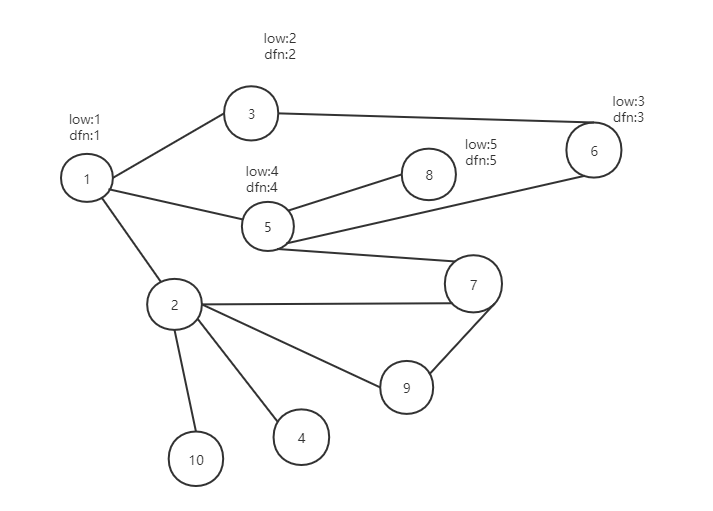
\includegraphics[scale=0.45]{picture1.png}
\end{figure}
首先由节点1作为起点进行深度优先遍历。如图所示,当访问到节点5时,有一已访问的邻节点1,于是在回退时更新5及所有父节点的low值。

\begin{figure}[ht]
\centering
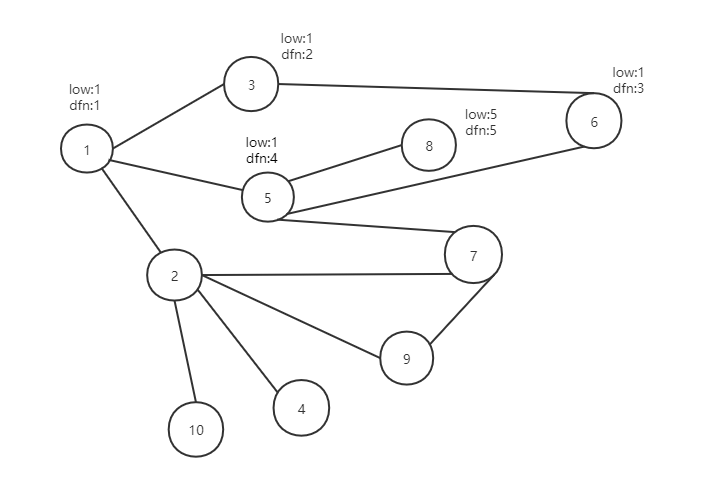
\includegraphics[scale=0.45]{picture2.png}
\end{figure}

该图是5节点及其父节点的low值更新之后的状态。在已经访问过的节点中,只有节点1和5满足存在一个儿子节点的low大于等于dfn值,因此节点1是割点。\\
\\

通过如上方式进行深度优先遍历,最后得到的图的结果是

\begin{figure}[ht]
\centering
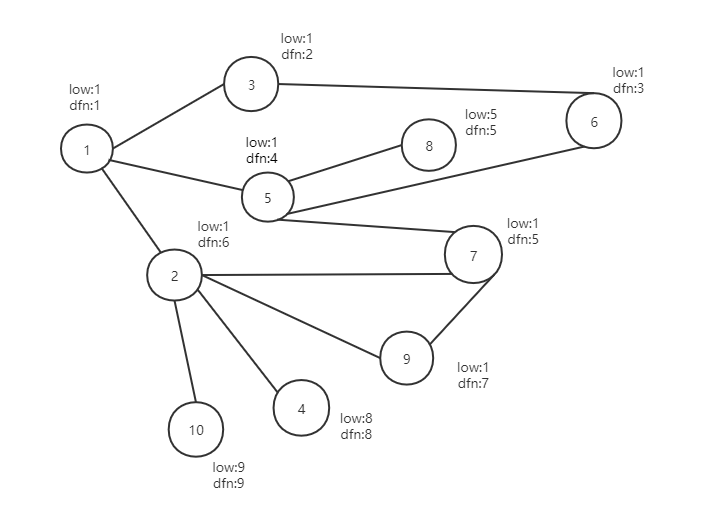
\includegraphics[scale=0.45]{picture3.png}
\end{figure}

满足子节点V和父节点U的$dfn[u]\ <\ low[v]$,则V-U是割边,在图中有2-10,2-4,5-8。因此割边共有3条。并且在余下的遍历中并没有新的割点出现,因此割点共有两个,为节点1,5。

\section{静态区间查询}
\subsection{本关任务}
给定一个长度为$N$的数列,和$M$次询问,求出每一次询问的区间内数字的最大值。
\subsection{解法}
设二维数组$dp[i][j]$表示的是区间$[i,\ j]$的最大值。

(1) $dp[ i ][ i ]\ =\ arr[ i ]$

(2)易得$dp[i][j+1]\ =\ max(dp[i][j],\ arr[j])$,迭代计算每一个dp值。

(3)读入一组区间,直接查询对应的dp数组值。
\subsection{分析与证明}
对于解法的第一步,初始化$n$个二维数组dp的值,串行复杂度为$O(n)$,并行复杂度为$O(1)$。
对于解法第二步,固定左区间端点更新dp数组,判断与更新都是串行的,Work和Span都是$O(n)$的复杂度。需要进行$n$个区间端点的更新,这里可以进行并行处理,因此该算法串行复杂度为$O(n^2)$,并行复杂度为$O(n)$。

设需要查找的次数为$M$,则查找过程的Work为$O(M)$,Span为$O(1)$。

得到$W=O(N^2+M),S=(N)$。

\begin{algorithm}
  \SetAlgoLined
  MAX($L, R$) =\par
    \LetIn{
    $\langle dp[i][j]=0\ :\ 1\leq i\leq n,\ 1\leq j\leq n\rangle$\par
    $\langle dp[i][j]=max\{dp[i][j-1],\ arr[j]\}\ :\ 1\leq i\leq n,\ i\leq j\leq n\rangle$
    }{$dp[L][R]$}
  \caption{MAX}
\end{algorithm}
\subsection{样例结果与输出}
样例输入:

8 8

9 3 1 7 5 6 0 8

1 6

1 5

2 7

2 6

1 8

4 8

3 7

1 8

样例输出:

9 9 7 7 9 8 7 9

样例分析:

对于左端点从1开始的情况来说,记录最大值。dp[1][1]=9,dp[1][2]=max{dp[1][1],arr[2]}。


得到结果:$dp\left[1\right]:\left[9,9,9,9,9,9,9,9\right]$

同理:$dp\left[2\right]:\left[0,3,3,7,7,7,7,7\right]$

$dp\left[3\right]=...$

再对每一组区间$\left[L,\ R\right]$进行查询,结果就等于$dp\left[L\right]\left[R\right]$。
\section{素性测试}
\subsection{本关任务}
给定一个数$N$,判断它是否是素数。
\subsection{解法}
利用Miller-Rabin算法来判断数字是否是素数。

该算法是对下面两个定理进行应用:

$\ \ \ \ $	1.费马小定理:当$p$为质数时,有$a^{p-1}\equiv 1(mod\ p)$。

$\ \ \ \ $	2.二次探测:如果$p$是一个素数,$0\ < x\ < p$,则方程$x^2\equiv 1(mod\ p)$的解为$x\ =\ 1$或$x\ =\ p\ -\ 1$。

算法流程如下:

输入一个数$x$。

(1)当$x$是偶数可以直接判断。

(2)当$x$是奇数时,选择一个比较小的质数$a$,并计算$2^s\cdot t\ =\ x\ -\ 1$。

(3)先算出$a^t$(由于$a^t$的值可能非常大,因此只需要算出$a^t\ mod\ x$就可以了),然后进行$s$次平方进行二次探测的循环。如果在循环中,当前数的平方模$x$与1同余并且该数不等于$1$或$x-1$,那么$x$就是合数,直接退出循环。

(4)根据费马定理判断$a^{p-1}\equiv 1(mod\ p)$是否成立。如果成立,说明该数很有可能是合数,为了增加正确性,可以从第(2)步挑选其它质数$a$再次判断。
\subsection{分析与证明}
时间复杂度分析:

若$x$是偶数,那么可以直接判断,复杂度为$O(1)$。

若$x$是奇数,第二步需要的时间复杂度为$O(logn)$。在进行第三步时,平方取余数,再通过二次探测的操作判断。共需要进行$O(logn)$次循环,每一次循环需要判断是否与$x$同余,共需要$O(logn)$的复杂度。最后一步利用费马定理判断也是$O(logn)$的复杂度。因此总的时间复杂度为$O(log^2)$。如果共选择了$k$个素数进行分析,则所有步骤的时间复杂度为$O(klog^2n)$。

空间复杂度分析:

在算法中只需要储存需要判断的数字,和在循环中进行平方的$a^{k}\cdot t(k=0,1,2,...,n)$的数。而在实际实现时需要在平方之后直接取模,为了保证计算的正确性又是保证计算的速度。因此此算法的空间复杂度仅由输入的数字决定,时间复杂度为$O(1)$。




\subsection{样例结果与输出}

样例输入:

100003

样例输出:

True

样例分析:

首先取质数$a\ =\ 3$进行试探。

根据步骤(2),求出满足$3^s\cdot t\ =\ x\ -\ 1$的解为$t\ =\ 50001, s\ =\ 1$。$a^t\ mod\ =\ 3^50001\mod x\ =\ 100002$。进行第一次探测,$100002^2$模$x$与1同余,并且$100002\ =\ x\ =\ 1$,因此符合条件,因为$s=1$,探测结束。并且该数符合费马小定理,因此100003很有可能是质数。使用同样方法,取不同的质数进行判断,可以说明100003是质数。
\end{document}
